\documentclass[twocolumn,aps,prd,superscriptaddress]{revtex4-1}  
\usepackage{amsmath,graphicx}

\DeclareMathOperator{\Tr}{Tr}

\usepackage[usenames]{color}
\newcommand{\CiteNeed}{\textcolor{red}{\scriptsize[citation needed]}}
\newcommand{\sv}[1]{\textcolor{blue}{\it{\textbf{sv: #1}}} }
\newcommand{\ki}[1]{\textcolor{cyan}{\it{\textbf{ki: #1}}} }

\newcommand{\Agw}{\ensuremath{A_\mathrm{gw}}}


\begin{document}

\title{Assessing spatial correlations in pulsar timing arrays with the noise-marginalized optimal statistic}


\author{Sarah J.\ Vigeland}
\affiliation{Center for Gravitation, Cosmology and Astrophysics, University of Wisconsin--Milwaukee, PO Box 413, Milwaukee WI, 53201, USA}

\author{Kristina P.\ Islo}
\affiliation{Center for Gravitation, Cosmology and Astrophysics, University of Wisconsin--Milwaukee, PO Box 413, Milwaukee WI, 53201, USA}

\author{Stephen R.\ Taylor}
\affiliation{Jet Propulsion Laboratory, California Institute of Technology, 4800 Oak Grove Drive, Pasadena, California 91106, USA}

\author{Justin A.\ Ellis}
\affiliation{Jet Propulsion Laboratory, California Institute of Technology, 4800 Oak Grove Drive, Pasadena, California 91106, USA}

\date{\today}  

\begin{abstract}
Supermassive black hole binaries (SMBHBs) are predicted to form a 
high-redshift cosmological population of low-frequency gravitational wave sources 
which added together produce a stochastic gravitational wave background (GWB) 
that can be observed by pulsar timing arrays (PTAs). 
Comparing the actual and predicted times-of-arrival (TOAs) of radio pulses beamed by 
millisecond pulsars allows us to search for and place limits on the stochastic background. 
While most estimating of GWB significance is done via Bayesian analysis, 
here we use a frequentist estimator called the noise-marginalized optimal statistic 
to assess the significance of a GWB present in simulated PTA data. We find \ki{complete}

Test travis

\end{abstract}

\maketitle


\section{Introduction}

Low-frequency gravitational waves (GWs) with frequencies of 
$10^{-9} - 10^{-7} \; \mathrm{Hz}$ can be observed with pulsar timing arrays (PTAs) 
composed of millisecond pulsars (MSPs) \cite{hd1983,fb1990}. 
The dominant astrophysical source in this frequency range is an isotropic stochastic 
gravitational wave background (GWB) 
made up of the incoherent superposition of GWs from inspiraling 
supermassive black hole binaries (SMBHBs) 
\citep{1995ApJ...446..543R, 2003ApJ...583..616J, 2003ApJ...590..691W}. 
By monitoring the ultra-regular periodic emission from these pulsars using radio telescopes, 
we can probe the dynamics of the spacetime through which the pulses travel. 
This is done by searching for correlations in the pulsar timing residuals, 
which measure the difference between the expected and observed pulse times of arrival. 
Current upper-limits on the stochastic background from PTAs are approaching 
theoretical predictions for the stochastic GWB \citep{PPTA2013,EPTA2015,NANOGrav9yr}

The primary data analysis technique used by PTAs is Bayesian inference 
to compare the probabilities of various models for the pulsar timing residuals, 
including one where the residuals contain evidence of an isotropic GW stochastic background 
\citep{vlm+2009,lah+2013}. 
Bayesian inference is a powerful technique because it allows us to compare arbitrarily complicated models. 
However, running a full Bayesian analysis is computationally intensive, 
particularly when searching for evidence of dipole spatial correlations -- 
``the smoking gun'' of a stochastic GWB.

The significance of a stochastic GWB can also be assessed using the 
optimal statistic, a frequentist estimator for the GWB amplitude \citep{abc+2009,demorest+2013,ccs+2015}. 
It is an important complement to Bayesian detection techniques 
because it provides an independent detection procedure, 
and it is significantly faster to compute. 
In particular, different spatial correlations can be tested with the optimal statistic 
in less than a second, 
whereas a Bayesian analysis with spatial correlations requires 
several weeks to run on a supercomputing cluster.

However, previous work has found that the optimal statistic gives biased results 
for PTAs with significant red noise in the individual pulsars due to the 
strong covariance between the individual red noise parameters 
and the GWB amplitude \sv{has this ever been discussed in a paper?}. 
In this paper, we present a technique for improving the accuracy of the optimal statistic 
by marginalizing the optimal statistic over the individual red noise parameters 
using the posterior distributions from a full Bayesian analysis. 
This hybrid approach produces a more accurate 
estimate of \Agw\ and its uncertainty. 
This method is more computationally intensive than previous methods 
for computing the optimal statistic, but still requires only minutes. 
Furthermore, the same Bayesian analysis drawn upon by the noise marginalization 
can be used to compute the optimal statistic with any choice of the ORF, 
allowing additional spatial correlations to be tested very quickly.

This paper is organized as follows. In Sec.~\ref{sec:marg_os} 
we lay out the procedure for computing the noise-marginalized optimal statistic 
and compare to the fixed-noise optimal statistic. 
In Sec.~\ref{sec:spatial} determine how well 
the noise-marginalized optimal statistic can 
differentiate between different spatial correlations 
using simulated PTA data. 
In Sec.~\ref{sec:skyscrambles} we determine how well the noise-marginalized optimal statistic 
can assess the significance of a GW detection by performing sky scrambles \citep{cs2016}. 
We also compare our sky scramble results to the Bayesian analysis of sky scrambles done by \citet{tlb+2017}. 
We conclude in Sec.~\ref{sec:conclusion}.


\section{Noise-marginalized optimal statistic}
\label{sec:marg_os}

\sv{Justin, please bring notation up to date}
As introduced by \citet{abc+2009}, 
the optimal statistic is derived by analytically maximizing 
the PTA likelihood function in the weak-signal regime. 
We begin by finding the timing residuals for a given pulsar ${\bf{r}}_I$, which can be written as 
\begin{equation}
	{\bf{r}}_I = M {\bf{\epsilon}}_I + F {\bf{a}}_I + U {\bf{j}}_I + {\bf{n}}_I \,,\\
\end{equation}
where $M$ is the design matrix, 
$\epsilon_I$ is a vector of the timing model parameter uncertainties, 
${\bf{a}}_I$ are the red noise parameters describing both individual pulsars' red noise 
and common red noise in all pulsars, 
${\bf{j}}_I$ are white noise parameters describing frequency-correlated white noise, 
and ${\bf{n}}_I$ are white noise parameters describing uncorrelated white noise. 
The likelihood function is constructed from the residuals as given by
\begin{equation}
	p({\bf{r}}|\phi) = \frac{\exp[-\frac{1}{2} {\bf{r}}^T \Sigma^{-1}(\phi) {\bf{r}} ]}{\sqrt{\mathrm{det}[2\pi \Sigma(\phi)]}} \,,
\end{equation}
where $\bf{r}$ is an array of the timing residuals 
from the $M$ pulsars in the PTA,
\begin{equation}
	\bf{r} = \left[ \begin{array}{c} {\bf{r}}_1 \\ {\bf{r}}_2 \\ \vdots \\ {\bf{r}}_M \end{array} \right] \,,
\end{equation}
$\phi$ is the set of pulsar noise parameters, 
and $\Sigma$ is the covariance matrix of the residuals. 
We can write $\Sigma$ in terms of 
autocovariance and cross-covariance matrices ${\bf{P}}_I$ and ${\bf{S}}_{IJ}$, respectively, as
\begin{equation}
	\Sigma = \left[ \begin{array}{cccc} {\bf{P}}_1 & {\bf{S}}_{12} & \hdots & {\bf{S}}_{1M}  \\
							{\bf{S}}_{21} & {\bf{P}}_2 & \hdots & {\bf{S}}_{2M} \\
							\vdots & \vdots & \ddots & \vdots \\
							{\bf{S}}_{M1} & {\bf{S}}_{M2} & \hdots & {\bf{P}}_M \end{array} \right] \,,
\end{equation}
where
\begin{eqnarray}
	{\bf{P}}_I &=& \left\langle {\bf{r}}_I {\bf{r}}_I^T \right\rangle \,, \\
	{\bf{S}}_{IJ} &=& \left. \left\langle {\bf{r}}_I {\bf{r}}_J^T \right\rangle \right|_{I \neq J} \,.
\end{eqnarray}
In the frequency domain, these can be written as
\begin{eqnarray}
	\left\langle {\bf{r}}_I {\bf{r}}_I^T \right\rangle_{ij} &=& {\bf{R}}_I \left[ \int_{-\infty}^\infty df \; e^{2\pi i f \tau_{ij}} P_I(f) \right] {\bf{R}}_I^T \,, \\
	\left. \left\langle {\bf{r}}_I {\bf{r}}_J^T \right\rangle \right|_{ij} &=& \chi_{IJ} {\bf{R}}_I \left[ \int_{-\infty}^\infty df \; e^{2\pi i f \tau_{ij}} P_\mathrm{gw}(f) \right] {\bf{R}}_J^T \,,
\end{eqnarray}
where $i,j$ index the matrix elements, $\tau_{ij} \equiv |t_i - t_j|$ is the time interval between 
two observations, 
$\mathbf{R}$ is the timing model fitting matrix, 
$\chi_{IJ}$ is the overlap reduction function (ORF) that describes the spatial correlation between two pulsars' residuals, 
$P_\mathrm{gw}(f)$ is the GW power spectrum, 
and $P_I(f)$ is the power spectrum for the $I$th pulsar. 

Analytically maximizing this likelihood gives the optimal statistic,
\begin{equation}
	\hat{A}^2 = \frac{\sum_{IJ} {\bf{r}}_I^T {\bf{P}}_I^{-1} \tilde{{\bf{S}}}_{IJ} {\bf{P}}_J^{-1} {\bf{r}}_J}{\sum_{IJ} \Tr \left( {\bf{P}}_I^{-1} \tilde{{\bf{S}}}_{IJ} {\bf{P}}_J^{-1} \tilde{{\bf{S}}}_{JI} \right) } \,,
\end{equation}
where $\tilde{{\bf{S}}}_{IJ}$ is the amplitude-independent cross-correlation matrix,
\begin{equation}
	\Agw^2 \tilde{{\bf{S}}}_{IJ} = {\bf{S}}_{IJ} \,.
\end{equation}
The normalization of $\hat{A}^2$ has been chosen so that 
$\langle \hat{A}^2 \rangle = \Agw^2$. 
For a weak GW signal, the standard deviation is 
\begin{equation}
	\sigma_0 = \left[ \sum_{IJ} \Tr \left( {\bf{P}}_I^{-1} \tilde{{\bf{S}}}_{IJ} {\bf{P}}_J^{-1} \tilde{{\bf{S}}}_{JI} \right) \right]^{-1/2} \,,
\end{equation}
and the signal-to-noise ratio (SNR) is
\begin{equation}
	\hat{\rho} = \frac{\hat{A}^2}{\sigma_0} = \frac{\sum_{IJ} {\bf{r}}_I^T {\bf{P}}_I^{-1} \tilde{{\bf{S}}}_{IJ} {\bf{P}}_J^{-1} {\bf{r}}_J}{\left[ \sum_{IJ} \Tr \left( {\bf{P}}_I^{-1} \tilde{{\bf{S}}}_{IJ} {\bf{P}}_J^{-1} \tilde{{\bf{S}}}_{JI} \right) \right]^{1/2}} \,.
\end{equation}
The expectation value of the SNR, averaged over all realizations of the stochastic background, is
\begin{equation}
	\left\langle \rho \right\rangle = \Agw^2 \left[ \sum_{IJ} \Tr\left( {\bf{P}}_I^{-1} \tilde{{\bf{S}}}_{IJ} {\bf{P}}_J^{-1} \tilde{{\bf{S}}}_{JI} \right) \right]^{1/2} \,.
\end{equation}

When constructing the residuals, 
we typically fix the red noise parameters to the values that 
maximize the likelihood. 
However, this leads to a bias in the optimal statistic and SNR because 
the individual red noise parameters and the common red noise parameters 
are highly covariant. 
In this section, we compare three different techniques for computing the 
optimal statistic for PTAs with significant red noise. 
First, we fix the individual pulsars' red noise parameters to the 
maximum-likelihood values from individual pulsar analyses. 
Second, we fix the individual pulsars' red noise parameters to the 
values maximum-likelihood values from a common analysis 
involving all of the pulsars in our PTA. 
For the third method, we draw values of the individual pulsars' 
red noise parameters from the posteriors generated by a Bayesian analysis 
that includes both individual red noise and a common red noise process, 
allowing us to marginalize over the individual red noise.

We used these three techniques to compute the optimal statistic for simulated data sets. 
We constructed simulated data sets using the same procedure as in \citet{tlb+2017}. 
The simulated PTAs consisted of 10 MSPs with 
total observation times and noise properties chosen to be 
similar to the properties of the EPTA \cite{caballero+2016} (see Table~\ref{tab:sim}). 
We also injected a stochastic GWB amplitude with $\Agw = 5\times10^{-15}$.
\begin{table}[htb]
	\setlength{\tabcolsep}{5pt}
	\caption{Pulsar parameters used in simulated PTA}
	\begin{center}
	\begin{tabular}{ccccc}
		\hline\hline
    		Pulsar	& $T_\mathrm{obs}$ (yrs) & $\sigma_w$ ($\mu\mathrm{s}$) & $\log_{10}A_\mathrm{red}$ & $\gamma_\mathrm{red}$ \\
		\hline
		J0613$-$0200 & 16.054 & 1.58 & -13.90 & 3.18 \\
		J0751+1807 & 17.606 & 2.60 & -14.14 & 2.58 \\
		J1012+5307 & 16.831 & 1.47 & -13.09 & 1.65 \\
		J1640+2224 & 16.735 & 1.99 & -13.24 & 0.03 \\
		J1643$-$1224 & 17.300 & 1.65 & -18.56 & 4.04 \\
		J1713+0747 & 17.657 & 0.26 & -14.90 & 4.85 \\
		J1744$-$1134 & 17.250 & 0.65 & -13.60 & 2.00 \\
		J1857+0943 & 17.310 & 1.51 & -16.00 & 1.35 \\
		J1909$-$3744 & 9.379 & 0.12 & -13.99 & 2.06 \\
		J2145$-$0750 & 17.161 & 1.19 & -13.87 & 4.02 \\
    		\hline\hline
	\end{tabular}
	\end{center}
	\label{tab:sim}
\end{table}

The optimal statistic was computed using the \sv{fill in...} in PAL2 \CiteNeed. 
Figure~\ref{fig:os_dataset_sample} shows the fixed-noise and noise-marginalized 
optimal statistic for a single realization of the stochastic background. 
We also include the distribution of $\Agw^2$ found using the results of a Bayesian analysis 
for a common red process. For this particular realization of the stochastic background, 
the values of $\hat{A}^2$ from the noise-marginalized and Bayesian analyses are in good agreement 
with each other and the injected GW stochastic background, 
but the value from the fixed-noise analysis is significantly lower. 
The noise-marginalized analysis also gives a larger mean SNR compared to the fixed-noise analysis.
\begin{figure}[ht]
	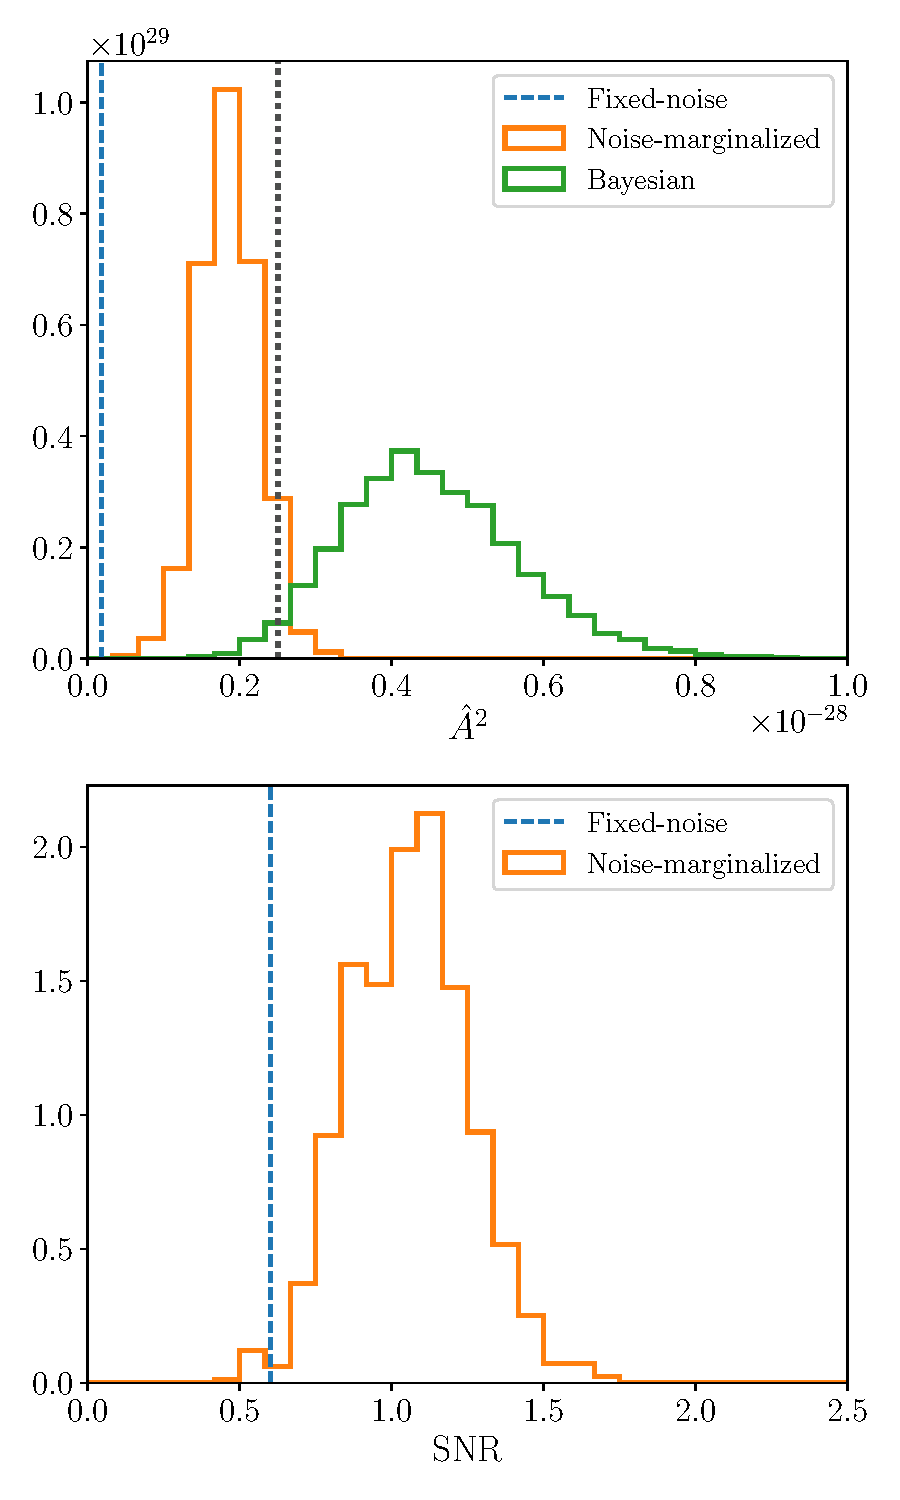
\includegraphics[width=0.9\columnwidth]{plots/os_dataset50.pdf}
	\caption{Optimal statistic and SNR for a simulated dataset 
			containing an injected GW background with $\Agw = 5\times10^{-15}$. 
			We compare the values found using a fixed-noise analysis (dashed blue line) to the 
			mean optimal statistic and mean SNR found by marginalizing over 
			the individual pulsars' red noise parameters (solid orange line). 
			We also include the distribution of $\Agw^2$ found using the results of a Bayesian analysis 
			for a common red process (solid green line). 
			The dotted vertical line indicates the injected value, $\hat{A}^2 = 2.5 \times 10^{-29}$. 
			For this particular realization of the stochastic background, the fixed-noise analysis 
			gives $\hat{A}^2 = 1.9 \times 10^{-30}$ with $\mathrm{SNR} = 0.60$, 
			while the noise-marginalized analysis gives $\hat{A}^2 = 1.9\times10^{-29}$ with $\mathrm{SNR} = 1.1$. 
			For comparison, the Bayesian analysis gives a mean value of $\Agw^2 = 4.5\times10^{-29}$.}
	\label{fig:os_dataset_sample}
\end{figure}

In Fig.~\ref{fig:os_datasetstats} we compare the fixed-noise values of $\hat{A}^2$ 
to the mean $\hat{A}^2$ for 425 different realizations of the stochastic background. 
The fixed-noise analysis tends to underestimate the strength of the stochastic background, 
whereas the noise-marginalized analysis is better able to recover the injected value. 
The mean value of the optimal statistic from the fixed-noise analysis, 
averaged over realizations of the stochastic background, is $\hat{A}^2 = 8.9 \times 10^{-30}$, 
while the mean value from the noise-marginalized analysis is $\hat{A}^2 = 2.5 \times 10^{-29}$. 
The noise-marginalized analysis also gives a higher average mean SNR of 1.7, 
compared to an average SNR of 1.0 using the fixed-noise analysis.
\begin{figure}[ht]
	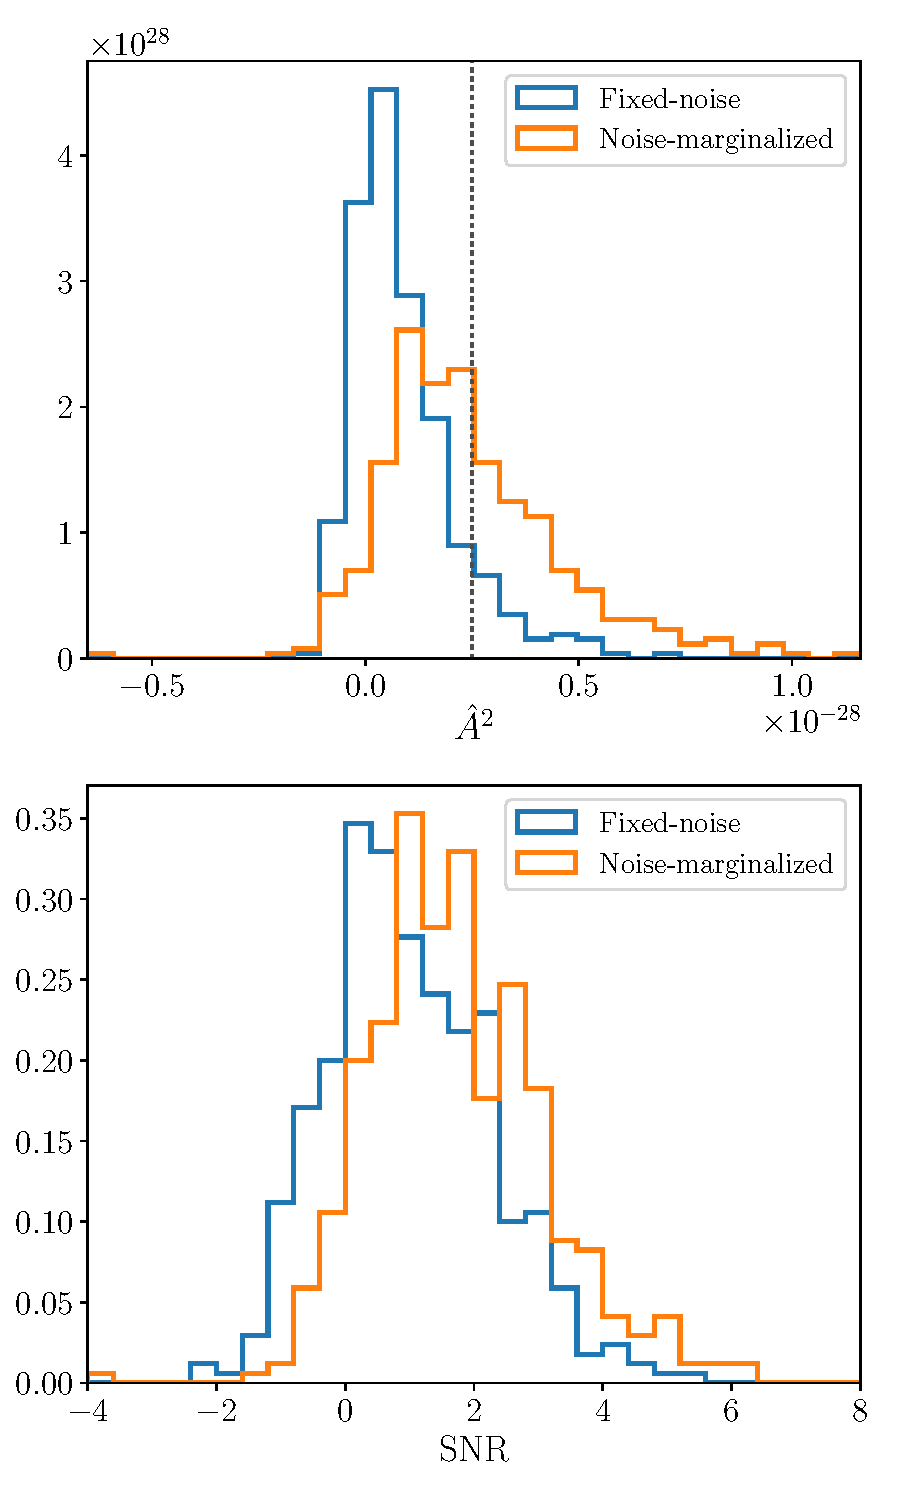
\includegraphics[width=0.9\columnwidth]{plots/os_datasetstats_5e-15.pdf}
	\caption{Optimal statistic and SNR for 425 simulated datasets 
			containing an injected GW background with $\Agw = 5\times10^{-15}$. 
			We compare the values found using a fixed-noise analysis (blue) to the 
			mean optimal statistic and mean SNR found by marginalizing over 
			the individual pulsars' red noise parameters. The dashed vertical line 
			indicates the injected value, $\hat{A}^2 = 2.5 \times 10^{-29}$. 
			The value of $\hat{A}^2$ from the fixed-noise analysis, 
			averaged over realizations of the stochastic background, is $\hat{A}^2 = 8.9 \times 10^{-30}$, 
			while the noise-marginalized analysis gives a mean value of $\hat{A}^2 = 2.5 \times 10^{-29}$. 
			Furthermore, the fixed-noise analysis gives an average SNR of 1.0, while the 
			noise-marginalized analysis gives an average mean SNR of 1.7.}
	\label{fig:os_datasetstats}
\end{figure}


\section{Monopole and Dipole Spatial Correlations}
\label{sec:spatial}

The optimal statistic is particularly well-suited to compare multiple spatial correlation relations 
because using a different spatial correlation only requires changing the ORF 
in $\tilde{{\bf{S}}}_{IJ}$. 
\citet{thk+2016} demonstrated how the optimal statistic can be altered to fit for 
multiple spatial correlations at once in order to mitigate common noise sources such as 
clock error and ephemeris error. 
Here we compute the optimal statistic with monopole and dipole spatial correlations 
for the same simulated data sets as in the previous section in order to determine 
how well we can distinguish a GW background from a monopole or dipole signal. 
For a monopole signal, the ORF becomes simply
\[ \Gamma(\theta_{IJ}) = 1 \,\]
while for a dipole signal, the ORF becomes
\[ \Gamma(\theta_{IJ}) = \cos\theta_{IJ} \,. \]

Figure~\ref{fig:os_ORF} shows the noise-marginalized mean value of $\hat{A}^2$ and the mean SNR 
computed assuming monopole, dipole, and quadrupole spatial correlations 
for 425 simulated data sets. Using a monopole or dipole ORF 
gives a lower value for the mean optimal statistic and mean SNR compared to the 
Hellings-Downs ORF. 
However, there is significant overlap between the distributions for the mean SNR using 
monopole, dipole, and quadrupole ORFs, indicating that it is not easy to differentiate 
between those three spatial correlations for an injected GW background of this amplitude. 
We find a noise-marginalized mean SNR above 1.0 in 68\% of our simulated data sets 
using the quadrupole ORF, and in 45\% and 24\% of our simulated data sets 
using the monopole and dipole ORFs, respectively.
\begin{figure}[htb]
	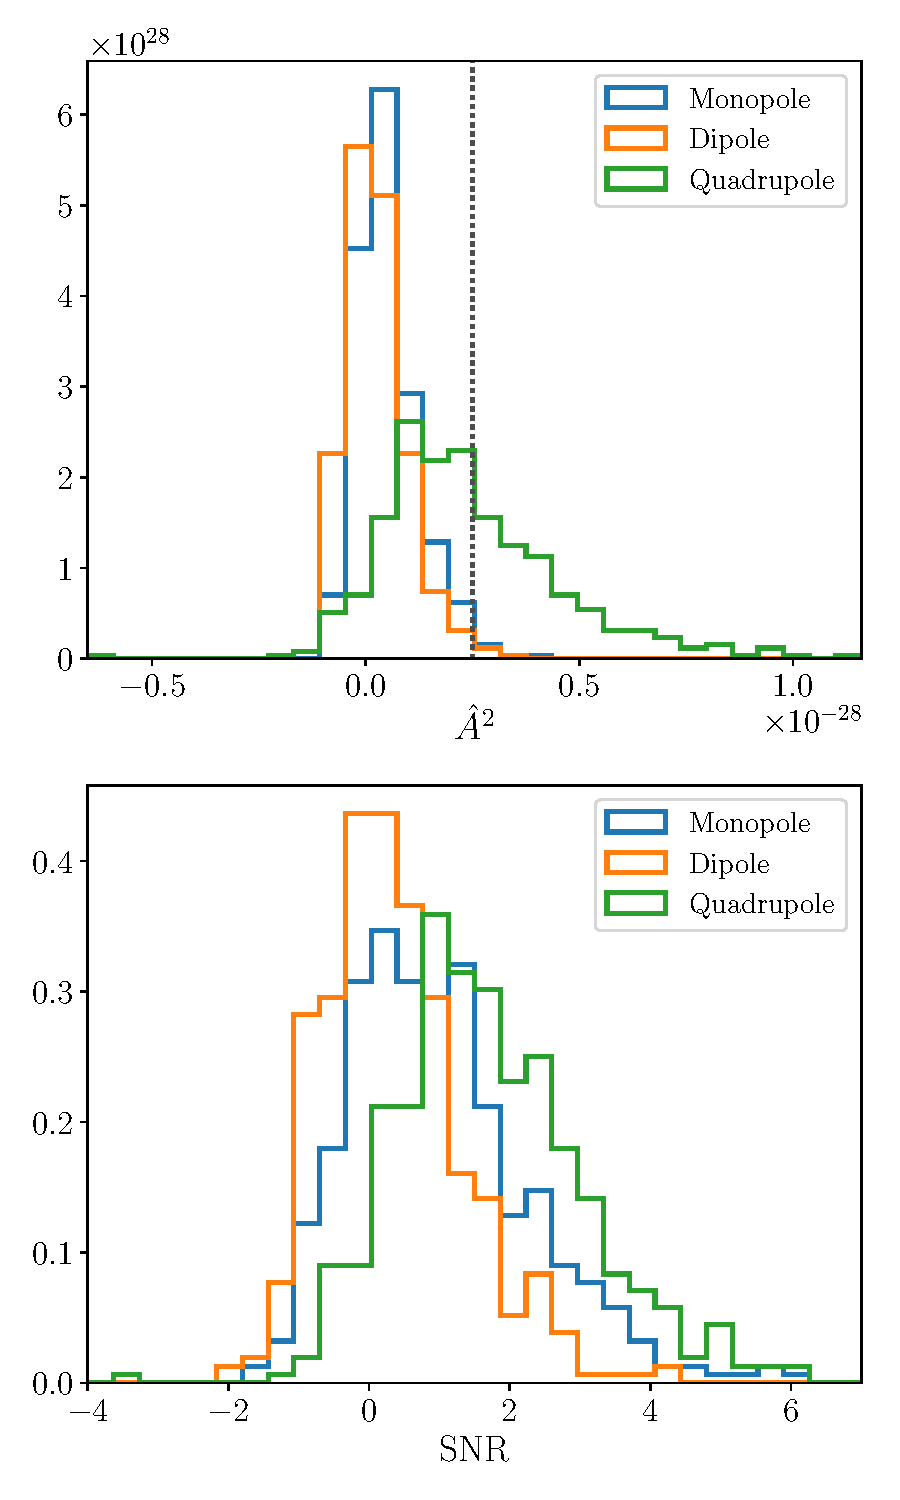
\includegraphics[width=0.9\columnwidth]{plots/os_datasetstats_5e-15_ORF.pdf}
	\caption{Noise-marginalized mean optimal statistic and mean SNR for 425 simulated datasets 
			containing an injected isotropic stochastic GWB with $\Agw = 5\times10^{-15}$. 
			We compare the values found using monopole (blue), dipole (orange), 
			and quadrupole (green) spatial correlations. 
			The dashed vertical line indicates the injected value, $\hat{A}^2 = 2.5 \times 10^{-29}$.}
	\label{fig:os_ORF}
\end{figure}


\section{Sky Scrambles}
\label{sec:skyscrambles}

Another technique for testing the spatial correlations is through ``sky scrambles,'' 
where the ORF is altered in order to simulate changing the pulsars' positions \citep{cs2016}. 
\citet{tlb+2017} showed how sky scrambles affect the Bayes' factor for simulated data sets. 
Here we perform a similar analysis using frequentist methods.

We used the same scrambled sky positions as were used in \citet{tlb+2017}. 
These positions were chosen so as to minimize the overlap  
between the scrambled ORFs and the true ORF, 
which can be assessed using the ``match statistic'' \citep{cs2016}:
\begin{equation}
	\bar{M} = \frac{\sum_{I,J \neq I} \Gamma_{IJ} \Gamma'_{IJ}}{\sqrt{ \left( \sum_{I, J \neq I} \Gamma_{IJ} \Gamma_{IJ} \right) \left( \sum_{I, J \neq I} \Gamma'_{IJ} \Gamma'_{IJ} \right)}} \,,
\end{equation}
where $I$,$J$ index the pulsar number, and $\Gamma$ and $\Gamma'$ are two different ORFs. 
The 210 sky scrambles used in this paper were generated 
using a particle swarm optimization (PSO) algorithm \citep{ke1995,se1998} 
with the requirement that the scrambled ORFs had $\bar{M} < 0.1$ when compared to the true ORF and to each other.
\sv{Steve, check this section}

Figure~\ref{fig:skyscrambles_dataset_sample} compares the noise-marginalized optimal statistic 
for a particular data set to the distribution of noise-marginalized optimal statistics obtained using sky scrambles. 
For this data set, the noise-marginalized mean optimal statistic is 
$1.9\times10^{-29}$ and the mean SNR is 1.1. 
The distributions of the noise-marginalized optimal statistic and SNR obtained using the scrambled ORFs 
are both centered around zero, 
and for 24 out of the 210 sky scrambles, the SNR is above the true value of $1.1$ ($p=0.11$). 
Figure~\ref{fig:skyscrambles} shows the $p$-values for 210 sky scrambles 
using 425 realizations of the stochastic background. 
For 62\% of simulations the $p$-value is $<0.1$, and for 29\% of simulations the $p$-value is $<0.01$.
\begin{figure}[htb]
	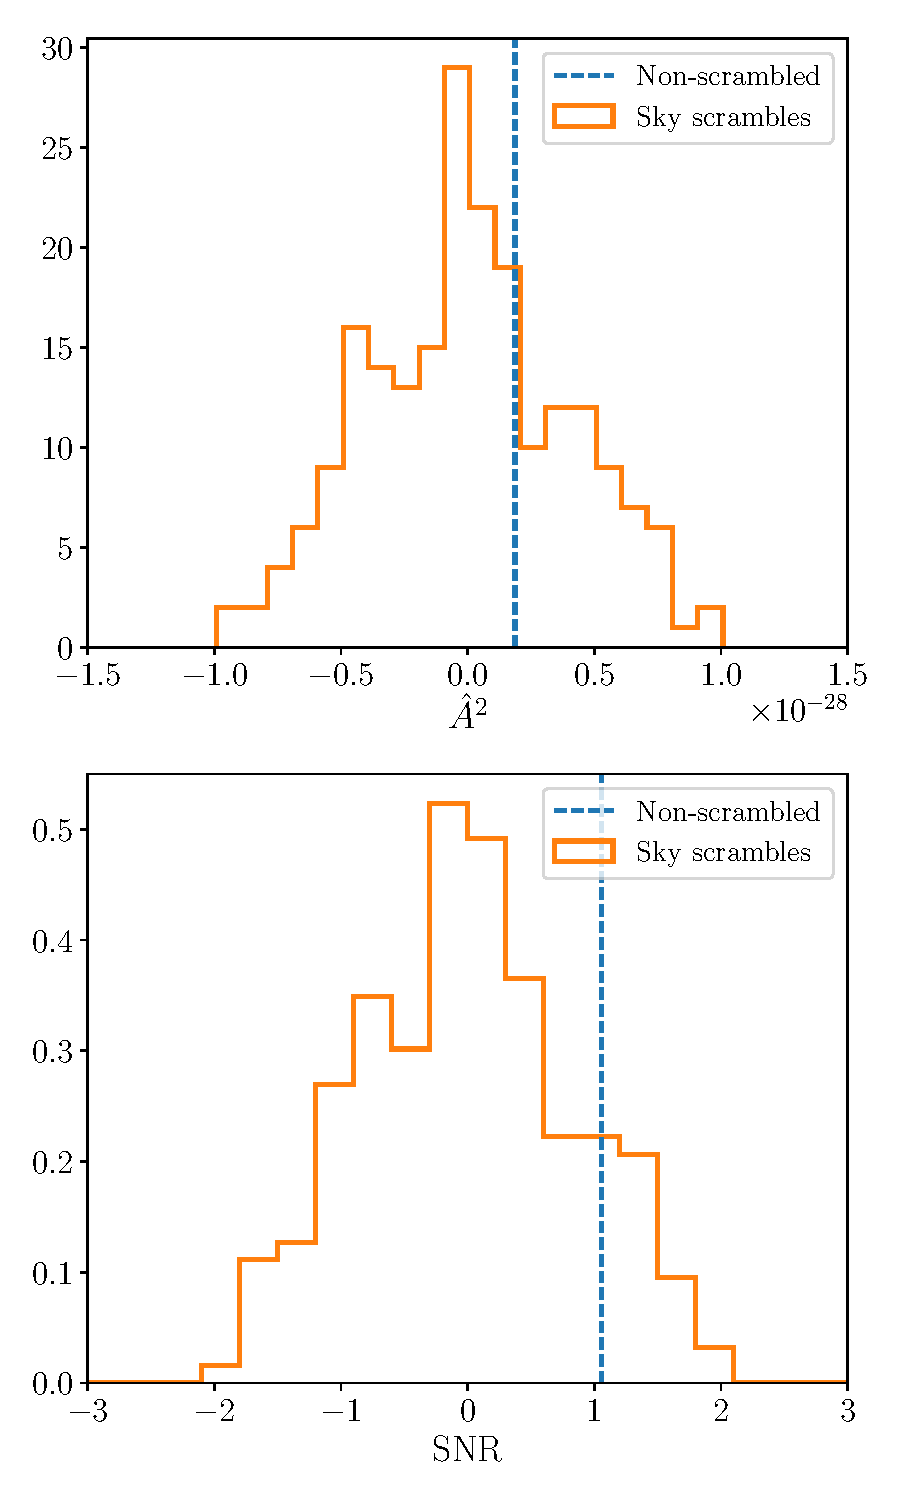
\includegraphics[width=0.9\columnwidth]{plots/skyscrambles_dataset50.pdf}
	\caption{Comparison between the noise-marginalized mean optimal statistic and mean SNR 
			with and without sky scrambles for a simulated dataset 
			containing an injected GW background with $\Agw = 5\times10^{-15}$. 
			Using the true ORF, we found an SNR of 1.1, while only 24 of the 210 analyses using scrambled ORFs 
			found an SNR $\geq 1.1$ ($p=0.11$).}
	\label{fig:skyscrambles_dataset_sample}
\end{figure}
\begin{figure}[htb]
	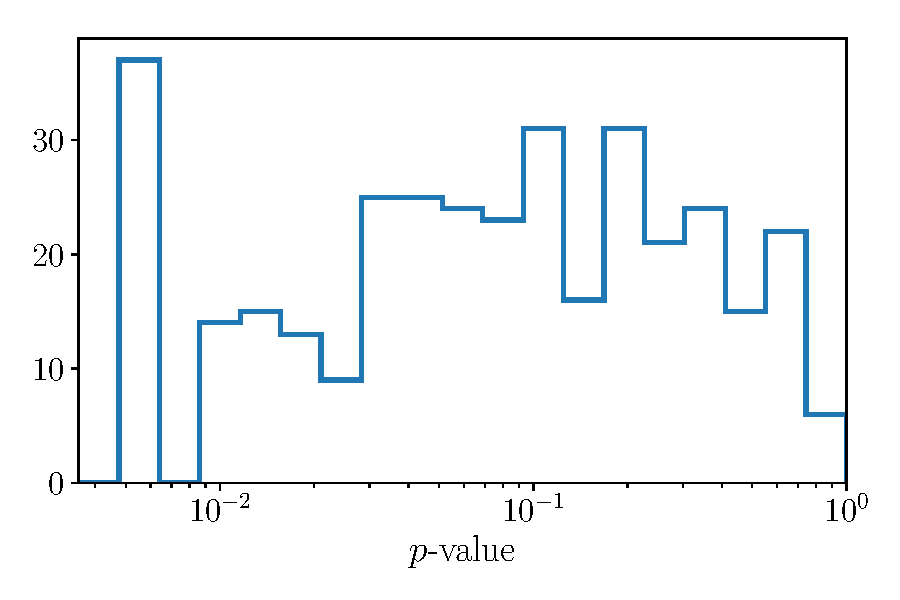
\includegraphics[width=0.9\columnwidth]{plots/os_skyscrambles.pdf}
	\caption{Distribution of $p$-values for 425 different realizations of the stochastic background. 
			For each realization, the $p$-value is the fraction of sky scrambled ORFs that gives a 
			noise-marginalized mean SNR greater than the mean SNR using the correct ORF.}
	\label{fig:skyscrambles}
\end{figure}

For five realizations of the stochastic background, we also computed the Bayes' factors for the 
true and sky scrambled ORFs in order to directly compare 
the frequentist and Bayesian detection techniques.
\sv{comparison to Steve's}


\section{Conclusion}
\label{sec:conclusion}

The noise-marginalized optimal statistic is a computationally inexpensive 
method for assessing the significance of an isotropic stochastic GWB in 
PTA data.


\acknowledgments
We thank Joe Romano and Xavier Siemens for useful discussions. 
KPI and SJV are supported by NSF Physics Frontier Center Grant 1430284.
JAE was supported by NASA through Einstein Fellowship Grant PF4-150120. 
SRT was supported by appointment to the NASA Postdoctoral Program 
at the Jet Propulsion Laboratory, which is administered by Oak Ridge Associated Universities 
and the Universities Space Research Association through a contract with NASA. 


\bibliographystyle{apsrev}
\bibliography{master}

\end{document}
